
	
	
	\begin{document}
		
		
		
	This section details the experimental implementation of an actively loaded differential amplifier with a common source output, cascoded current mirror and a class B amplifier stage at the output. These also include components for frequency compensation and a load.The power supplies and analysis were implemented using the Digilent Analog Discovery kit. The experimental circuit can be seen Figure \ref{fig:expercircuit}.
		
		
				
		\begin{figure}[H]
			\begin{center}
				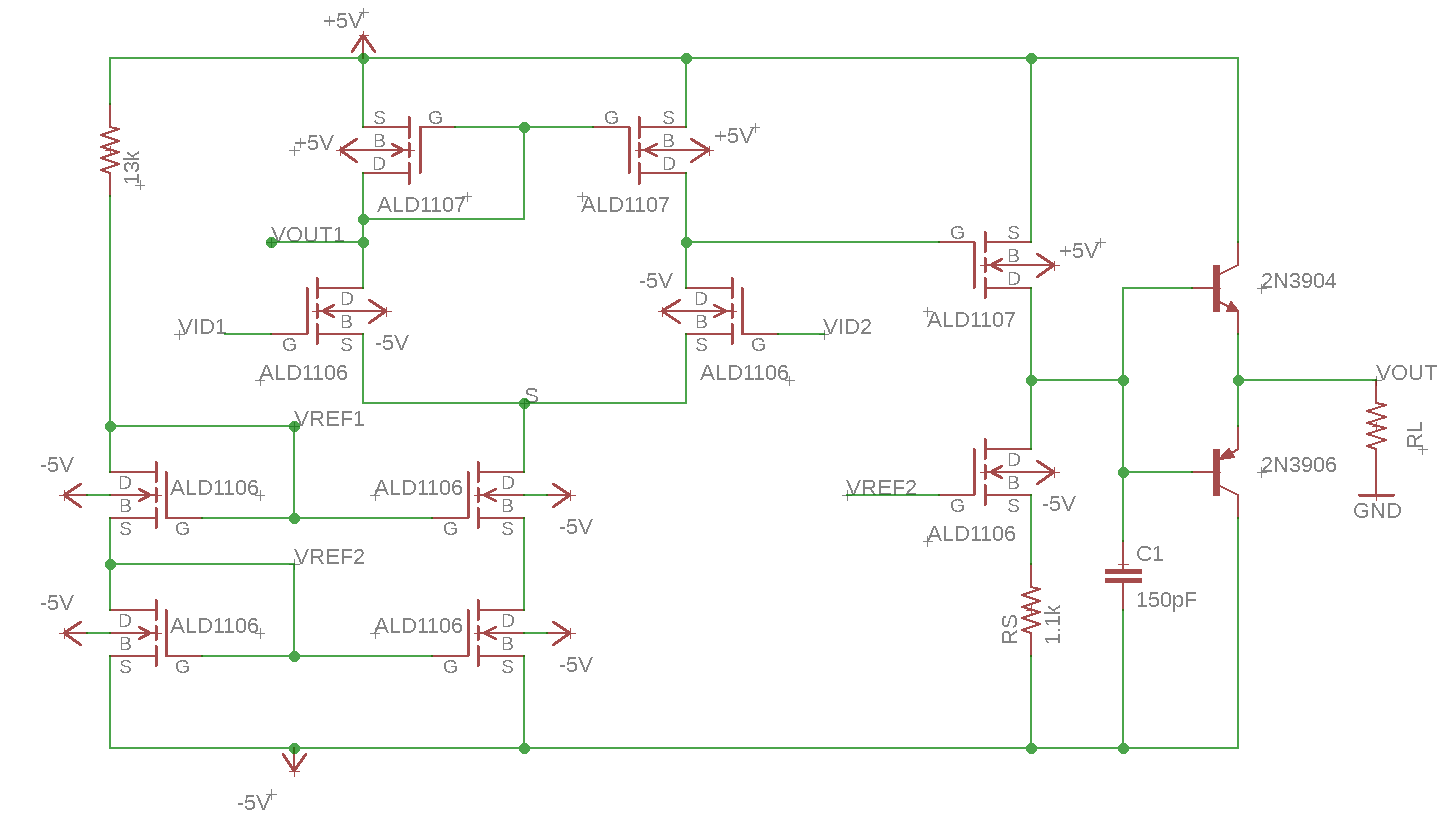
\includegraphics[scale=.40]{ExperimentalImplementation/expschem.png}
				\caption{Experimental range of operation}
				\label{fig:expercircuit}
			\end{center}
		\end{figure}

	
	The DC bias conditions were measured using a DT830B DVM. Nodal voltages were measured in reference to ground and current was measured by wiring the DVM in series while in ammeter mode. The bias conditions were measured while both input nodes to the circuit were grounded. The final measured values can be seen in Table \ref{tab:expdc}.
		
		
		\begin{table}[H]
			\centering
			\caption{Experimental DC values}
			\label{tab:expdc}
			\begin{tabular}{|l|l|}
				\hline
				\textbf{DC Bias Conditions} &           \\ \hline
				V$_{Ref_1}$                        & -3.01 V   \\ \hline
				V$_{Ref_2}$                        & -403 mV \\ \hline
				D1                          & 2.82 V     \\ \hline
				D2                          & 2.84 V     \\ \hline
				S                           & 2 V    \\ \hline
				OutCS                       & .09mV      \\ \hline
				I$_{Ref}$                        & 387 $\mu$A \\ \hline
				I$_{D_1}$                        &  193.7 $\mu$A\\ \hline
				I$_{D_2}$                        & 194 $\mu$A  \\ \hline
				I$_{CS}$  (CS stage)                      & 217 $\mu$A \\ \hline
				I$_{C}$   Collector                     & 2.23 $\mu$A \\ \hline
				
			\end{tabular}
		\end{table}
		
		Notably, the voltage at the "OutCS" node should be zero. In the default state, the offset at that node was measured to be 2.5V. A potentiometer was used as the source degeneration resistance for the common source amplifier. This pot was varied until the offset was nulled out and the final resistance value required was found to be 1.1k$\Omega$. The range of operation for the circuit can be seen in Figure \ref{fig:vtc}.
		
		
		\begin{figure}[H]
			\begin{center}
				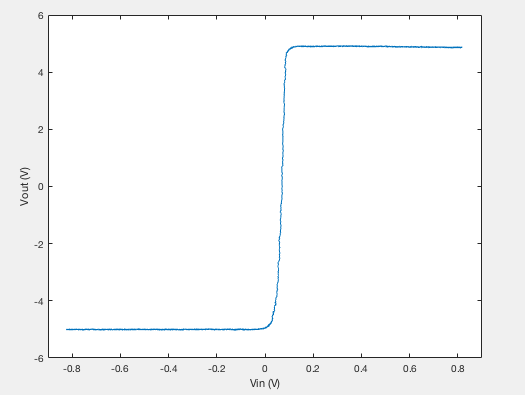
\includegraphics[scale=.40]{ExperimentalImplementation/VTC.png}
				\caption{Experimental range of operation}
				\label{fig:vtc}
			\end{center}
		\end{figure}
		
		The range of operation is extremely narrow. This, however, is expected due to the limits imposed by the use of a cascode current mirror. The cascode affords more gain at the expense of voltage range. This was explored in more depth in Task 3. In order to prevent the op amp from saturating, a 1000:1 voltage divider was added at the signal input. The channel 1 probe was connected after the voltage divider to compensate for the 60dB drop from the voltage divider. Channel 2 was connected at the final output of the operational amplifier. 
		
				\begin{figure}[H]
			\begin{center}
				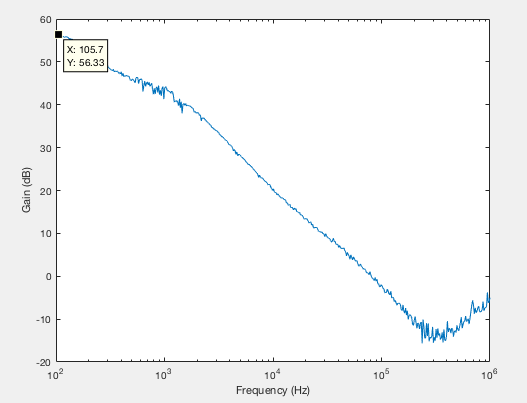
\includegraphics[scale=.40]{ExperimentalImplementation/gainwithload.png}
				\caption{Gain of loaded amplifier}
				\label{fig:gainwithload}
			\end{center}
		\end{figure}
	
	
			\begin{figure}[H]
		\begin{center}
			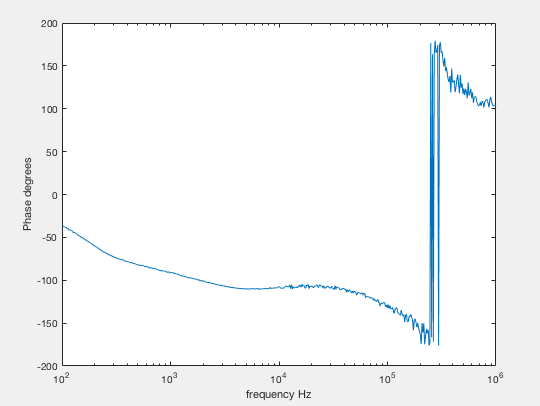
\includegraphics[scale=.40]{ExperimentalImplementation/phasewithload.png}
			\caption{Phase plot of loaded amplifier}
			\label{fig:phasewithload}
		\end{center}
	\end{figure}


		\begin{figure}[H]
	\begin{center}
		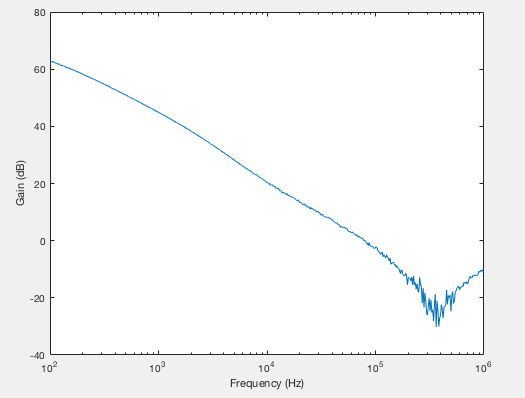
\includegraphics[scale=.40]{ExperimentalImplementation/gainwithcomp.png}
		\caption{Gain plot of loaded amplifier and frequency compensation}
		\label{fig:gainwithcomp}
	\end{center}
\end{figure}


		\begin{figure}[H]
	\begin{center}
		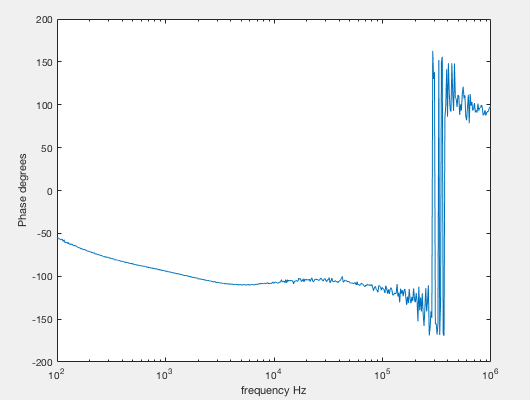
\includegraphics[scale=.40]{ExperimentalImplementation/phasewithcomp.png}
		\caption{Phase plot of loaded amplifier with frequency compensation}
		\label{fig:phasewithcomp}
	\end{center}
\end{figure}



		\begin{figure}[H]
	\begin{center}
		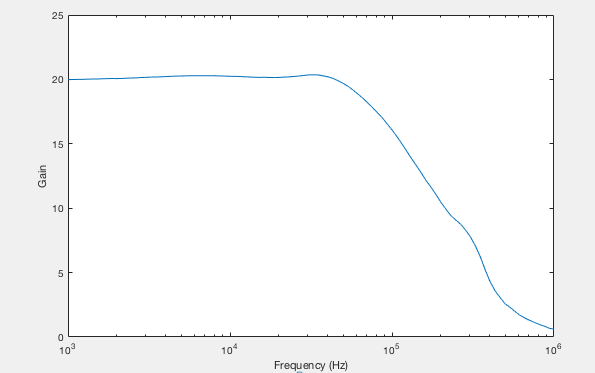
\includegraphics[scale=.40]{ExperimentalImplementation/invertingain.png}
		\caption{Gain of inverting amplifier}
		\label{fig:invertinggain}
	\end{center}
\end{figure}

		\begin{figure}[H]
	\begin{center}
		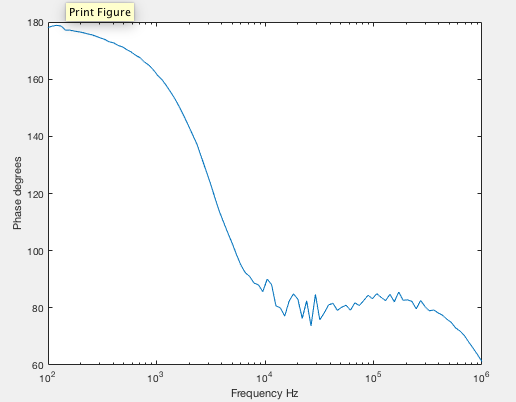
\includegraphics[scale=.40]{ExperimentalImplementation/invertingphase.png}
		\caption{Phase plot of inverting amplifier}
		\label{fig:invertingphase}
	\end{center}
\end{figure}
		
				\begin{figure}[H]
			\begin{center}
				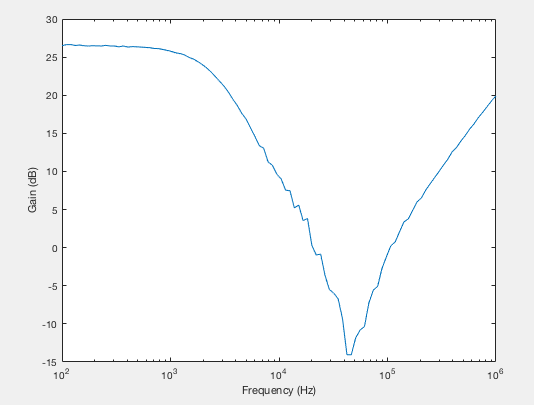
\includegraphics[scale=.40]{ExperimentalImplementation/gainnoninverting.png}
				\caption{Gain of non-inverting amplifier}
				\label{fig:gainnoninverting}
			\end{center}
		\end{figure}
	
			\begin{figure}[H]
		\begin{center}
			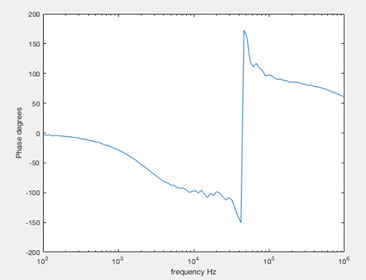
\includegraphics[scale=.40]{ExperimentalImplementation/phasenoninverting.png}
			\caption{Phase plot of non-inverting amplifier}
			\label{fig:phasenoninverting}
		\end{center}
	\end{figure}

		\begin{figure}[H]
	\begin{center}
		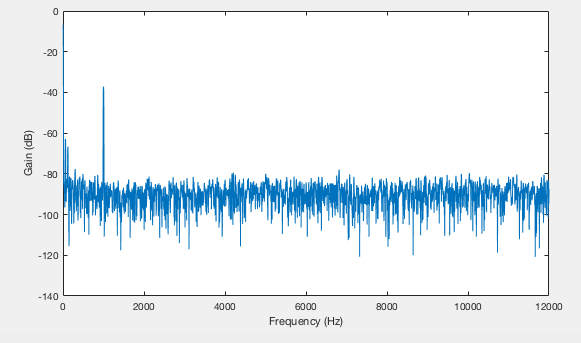
\includegraphics[scale=.40]{ExperimentalImplementation/spectrum.png}
		\caption{Harmonic spectrum of amplifier}
		\label{fig:spectrum}
	\end{center}
\end{figure}



	\end{document}
	